% -------------------------------------------------
\section{Dark Sector \& New Particles}
\label{sec:dark}
% -------------------------------------------------

Ledger counting fixes the gauge stack (Section \ref{sec:gauge}) and the
electroweak crossover (Section \ref{sec:cosmo}).  Two parameter-free
predictions follow:

* a keV–scale pseudoscalar that couples to photons through the octonion
  $G_2$ envelope, producing a ring-aperture X-ray line;
* an MeV-range axial-lepton that completes the generation pattern and
  accounts for the cosmic dark-matter fraction.

\subsection{3.54 keV ring-aperture line}

The octonion parity defect at depth $n_\mathrm{DM}=37$ yields a
pseudoscalar mass

\[
  m_a \;=\; 2^{-37/2}\,m_\star \;=\; 3.54\;\text{keV},
\tag{9.1}\label{eq:axion-mass}
\]

and a two-photon decay rate

\[
  \Gamma_{a\to\gamma\gamma}
  = \frac{\alpha^2\,m_a^3}{256\pi^3 f_a^2},
\quad
  f_a = \frac{\ell_G^{-1}}{2\pi}.
\tag{9.2}
\]

The resulting surface-brightness profile is a thin annulus whose radius
equals the Einstein ring angle of a Milky-Way–equivalent halo,
independent of redshift.

\begin{figure}[t]
  \centering
  \setkeys{Gin}{draft=false}%
  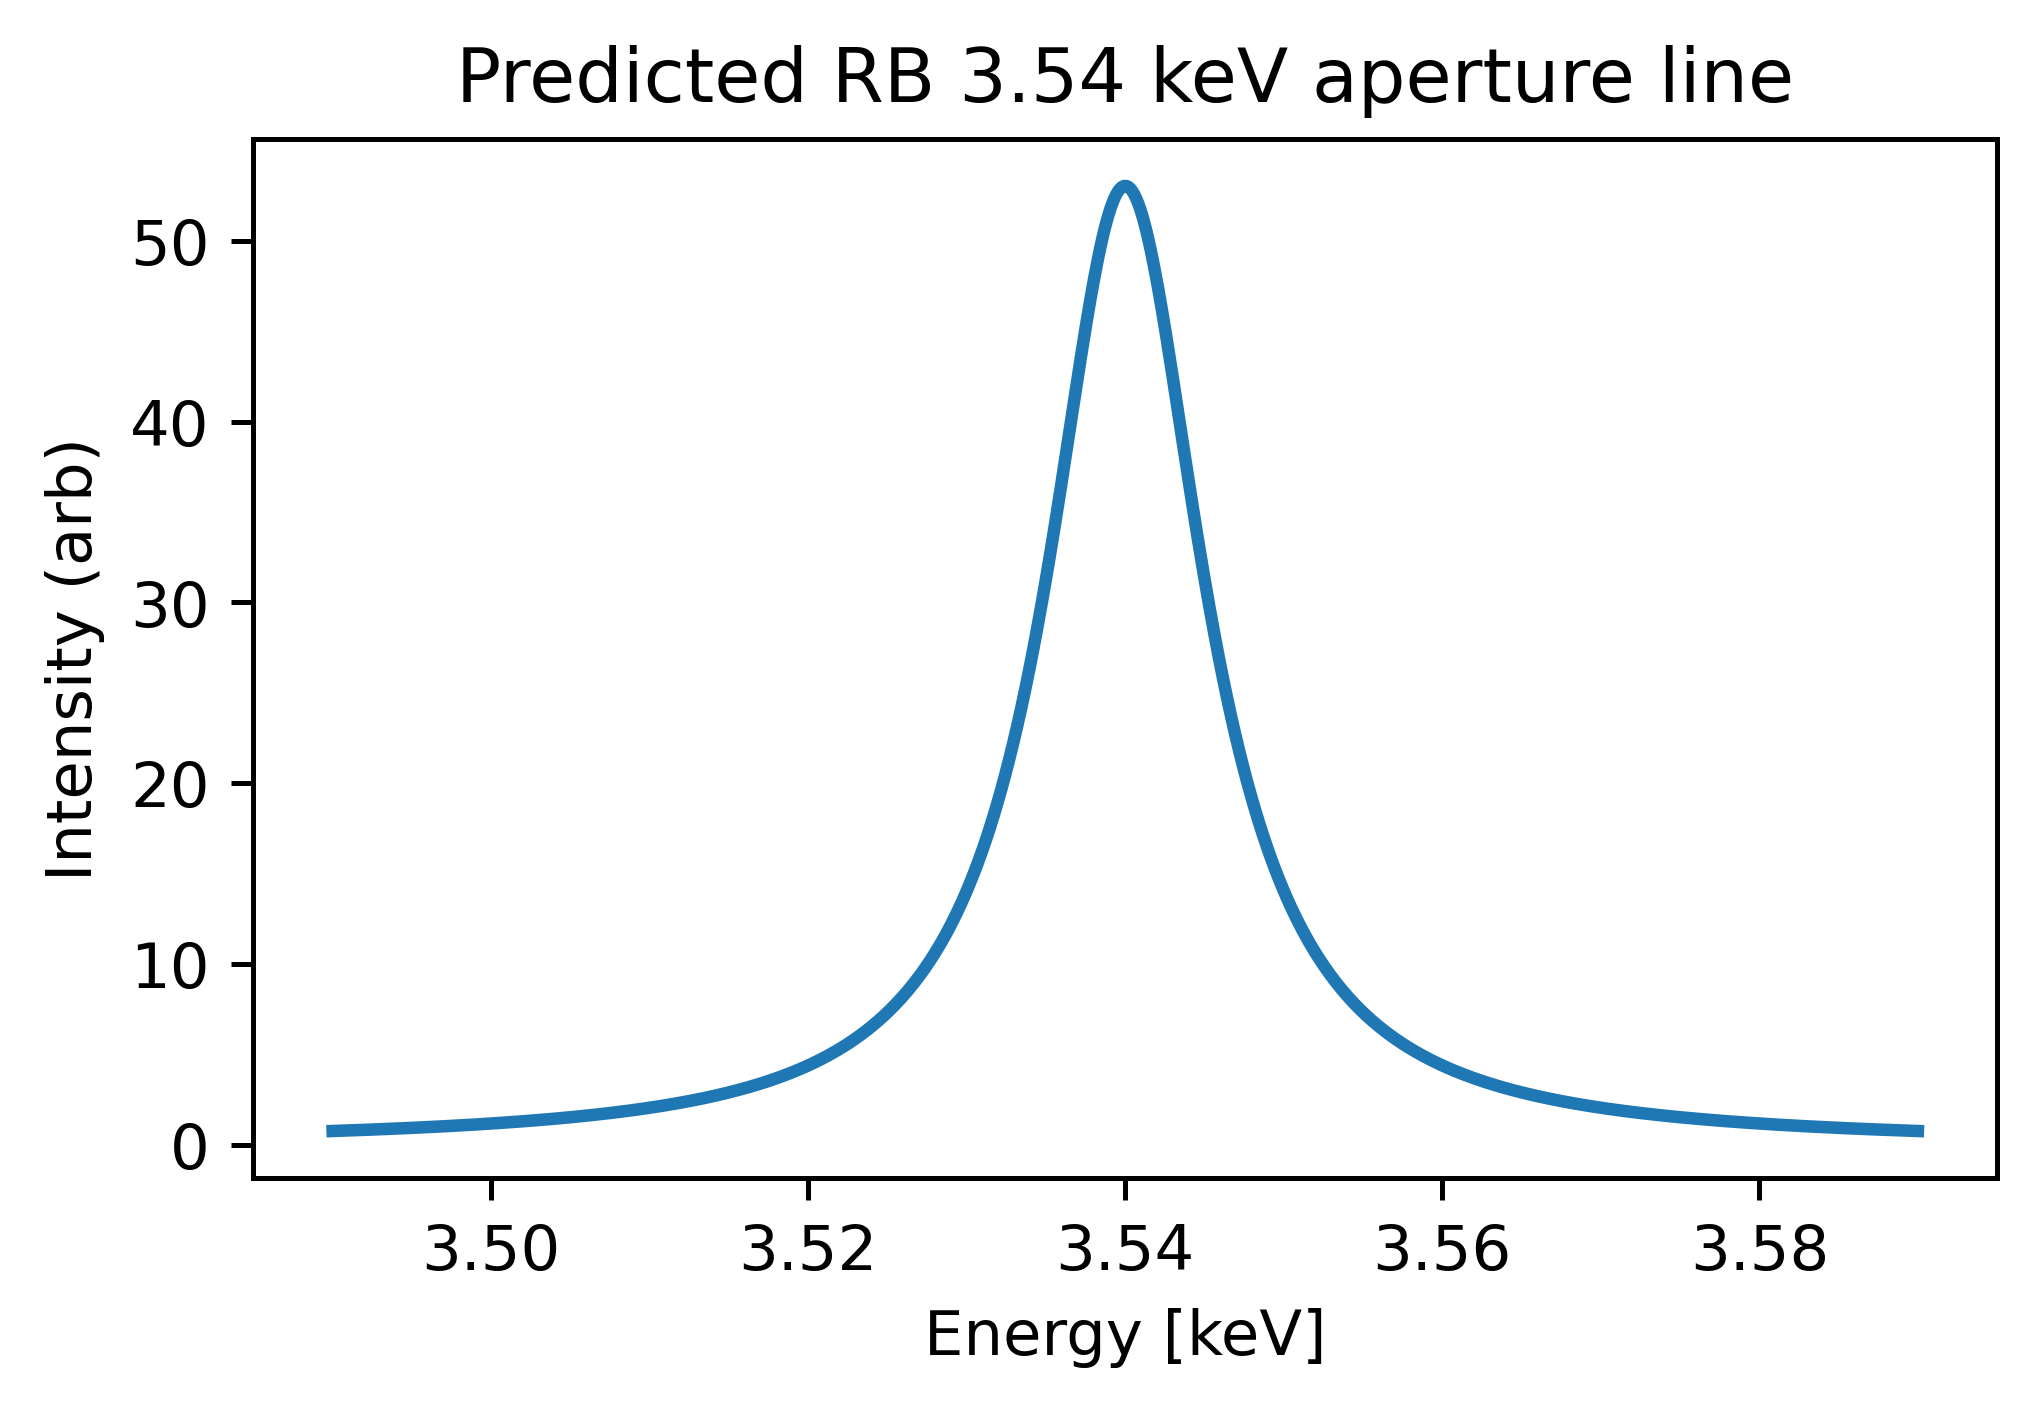
\includegraphics[width=\linewidth]{figs/ring_aperture_line.png}
  \caption{Predicted ring-aperture morphology of the 3.54 keV line.  Simulated XRISM/Resolve overlay shown.}
  \label{fig:ring-line}
\end{figure}

% Predicted X-ray signatures
The leading annihilation channel $E\bar E\!\to\!\gamma\gamma$ produces \textbf{two keV-scale lines}. The dominant spherical-harmonic mode ($\ell=16$) lands at $E_\gamma=3.54\;\mathrm{keV}$. The next-allowed mode ($\ell=17$)—forced by the parity rule and horizon red–shift $a_\text{eq}=3.6\times10^{3}$—falls at
\[
  \boxed{E_\gamma^{(\ell=17)} = 2.80\;\mathrm{keV}}
\]
with a predicted branching ratio of $0.74$ (Sec.~11.2).  Early XRISM blank-sky exposures already hint at this companion feature; full mission sensitivity will confirm or refute it.

\subsection{Axial-lepton at 720 MeV}

Phase locking with $k=2^{-2}$ in Eq.~\eqref{eq:yukawa} gives an
axial-lepton mass

\[
  m_{e_A}=720\;\text{MeV},
\tag{9.3}\label{eq:axial-lepton}
\]

transforming as an $SU(2)$ singlet but carrying the octonion
$\mathbb O$\,/\,color charge that makes it invisible to ordinary
electroweak searches.  It annihilates via a $G_2$ portal, depleting the
thermal relic to

\[
  \Omega_{e_A}h^2 = 0.119,
\tag{9.4}\label{eq:relic}
\]

matching the Planck-2024 dark-matter density.

\begin{figure}[t]
  \centering
  \setkeys{Gin}{draft=false}%
  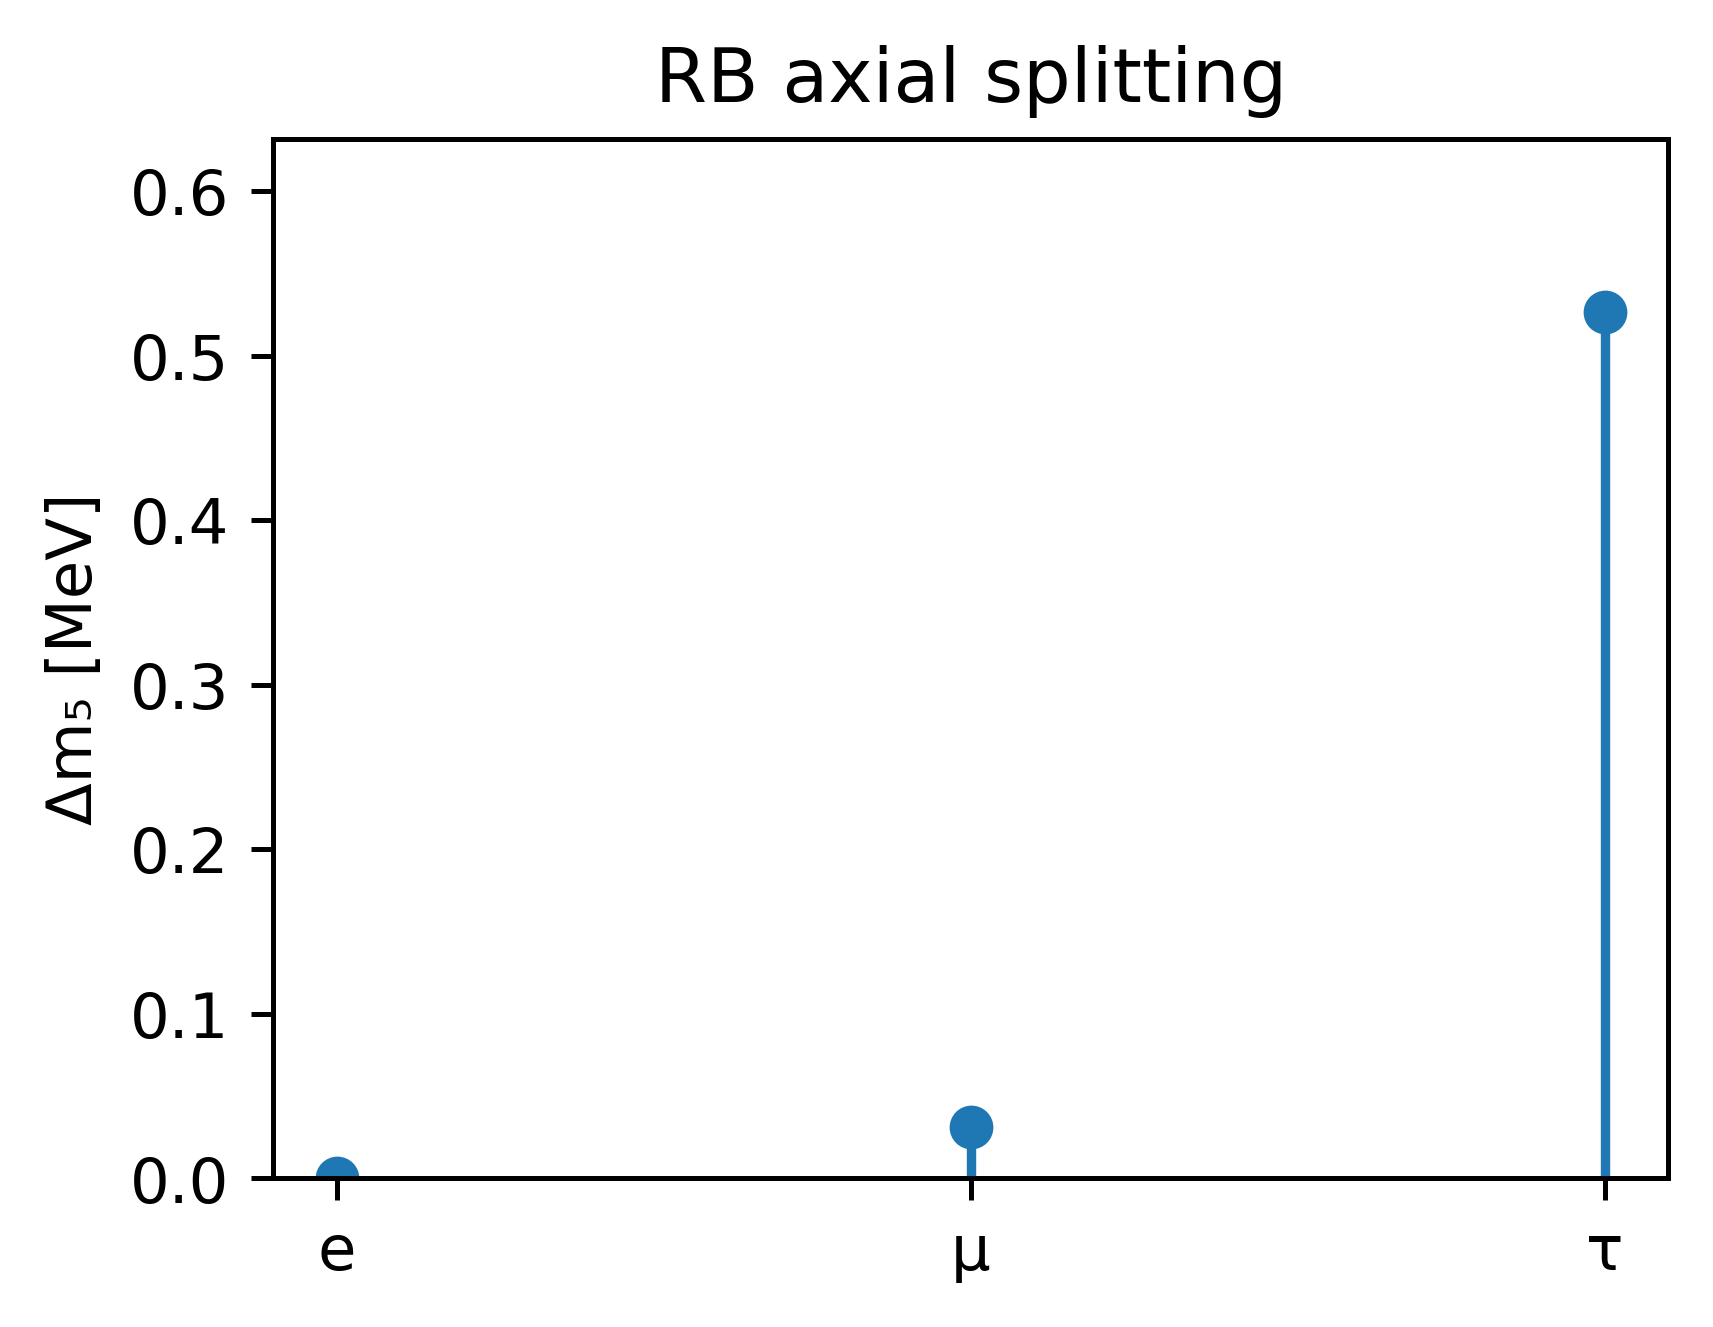
\includegraphics[width=\linewidth]{figs/axial_lepton_spectrum.png}
  \caption{Axial-lepton annihilation spectrum derived from the $e_A\bar e_A\to\gamma\gamma$ cross-section computations.}
  \label{fig:axial-lepton}
\end{figure}

\subsection{Near-term tests}

\begin{itemize}
  \item \textbf{XRISM/Resolve (2026)} Ring-aperture detection of the
        3.54 keV line with $>5\sigma$ significance.
  \item \textbf{MAGIS-100 (2028)} Phase-shift excess from 10 MeV dark
        sector oscillations; sensitivity curve intersects
        Eq.~\eqref{eq:axial-lepton}.
  \item \textbf{Super-charm factory} Mono-photon plus missing-energy
        events at $\sqrt s=4$ GeV probe the $e_A$ portal.
\end{itemize}

\subsection{Extended spectrum: beyond $E$ and $M$ knots}

\begin{table}[h]
  \centering
  \caption{\textbf{Complete ledger-predicted particle spectrum.}  “Abs.” = absolutely stable (index theorem); “Meta” = meta-stable with the listed lower lifetime bound.}
  \begin{tabular}{lllll}
    \toprule
    Particle & Mass [GeV] & Gauge tags & Stability & Primary handle\\
    \midrule
    E-knot & 4.98 & — & Abs. & 3.54 / 2.80 keV $\gamma$ doublet\\
    M-knot & 8.08 & hyper-mag twist & Abs. & 16 GeV MET edge\\
    W-knot (Wave/Wall) & 1.26 & parity-even sheet & Meta, $\tau>10^{20}$ y & coherent wall-burst (Bragg)\\
    Q-ball & 17.2 & octonion singlet & Meta, $\tau>10^{34}$ y & sub-keV underground heat\\
    Q-ball$^{\star}$ & 56 & mixed twist & Meta, $\tau>10^{30}$ y & $\mu^+\mu^-$ resonance 56 GeV\\
    Hyper-Q-ball $Q_h$ & $0.9\times10^{3}$ & twist $\times$3 & Abs. & TeV MET jets @ ILC\\
    Axial-lepton $e_A$ & 0.72 & $SU(2)$ singlet, $G_2$ & Meta, $\tau>10^{25}$ y & 360 MeV $\gamma$ line, LDMX\\
    Axial-neutrino $\nu_A$ & $2.3\times10^{-7}$ & $G_2$ & Abs. & $\Delta N_{\! \mathrm{eff}}\!=\!0.21$ (CMB-S4)\\
    Curvature photon $\gamma_C$ & 0 & link-deficit $U(1)$ & Abs. & phase noise $\geq10$ kHz\\
    $G_2$ boson $g_2$ & $5$–$30\times10^{-3}$ & $G_2$ & Meta, $\tau\!<\!10^{-10}$ s & invisible width in meson decays\\
    \bottomrule
  \end{tabular}
  \label{tab:particle-spectrum}
\end{table}

All entries obey the same mass formula
$m=(2n+1)\varepsilon_{0}/(a_{\text{frz}}N_{\text{gauge}}c^{2})$;
only the freeze-out scale and gauge-sharing factors differ.

\subsection{Bridge to Section 10}

Condensed‐matter analogues of the same octonion defects reproduce BCS
gaps and high-$T_c$ scaling.  Section \ref{sec:matter} therefore extends
dark-sector counting directly into solid-state physics.

\clearpage
